\documentclass[a4paper]{article}
\def\DOCTITLE{CSC3621 Cryptography}
% Set document attributes
\title{\DOCTITLE}

\usepackage{fullpage}
\usepackage{scrextend}
\usepackage{titlesec}
\usepackage{fancyhdr}
\usepackage{amsmath}
\usepackage{amssymb}
\usepackage[section]{placeins}
\usepackage{booktabs}
\usepackage{hyperref}
\usepackage{tikz}
\usepackage{graphicx}
\usepackage{minted}
\usepackage{subcaption}

% Setup headers and footers
\pagestyle{fancy}
\lhead{}
\chead{\DOCTITLE}
\rhead{}
\rfoot{}
\cfoot{\thepage}
\lfoot{}

% New page for each section
\newcommand{\sectionbreak}{\clearpage}

% Set header and footer sizes
\renewcommand{\headrulewidth}{0.4pt}
\renewcommand{\footrulewidth}{0.4pt}
\setlength{\headheight}{15.2pt}
\setlength{\headsep}{15.2pt}

\setlength{\parskip}{5pt plus 1pt minus 1pt}
\setlength{\parindent}{0pt}

% Newline after paragraph
\newcommand{\Para}[1]{\paragraph{#1}\mbox{}}

% Stuff used in cryptography notes
\newcommand{\Forall}{\;\forall\;}
\newcommand{\Mod}{\: mod \:}

% Stuff used in distributed systems notes
\newcommand{\happenbefore}{\rightarrow}
\newcommand{\orderbefore}{\Rightarrow}
\newcommand{\clockcond}{\leadsto}
\newcommand{\RArrow}{$\rightarrow$}

\def\checkmark{\tikz\fill[scale=0.4](0,.35) -- (.25,0) -- (1,.7) -- (.25,.15) -- cycle;}


\begin{document}

\tableofcontents

\section{Maths}

\subsection{Discrete Probability}

Given a finite sample space $S = \{s_{1}, s_{2}, \ldots, s_{n}\}$ the probability
$P$ on $S$ is $\{p_{1}, p_{2}, \ldots,p_{n}\}$ where:

\begin{align*}
  0 \leq p_{i} \leq 1 \\
  \sum_{i}p_{i} = 1
\end{align*}

\subsubsection{Events}

\begin{itemize}
  \item Event $E$ is a subset of $S$
  \item Complimentary event $\bar{E}$
  \item Probability of occurrence $P(E)$
  \item $P(E) = 1 - P(\bar{E})$
\end{itemize}

\subsubsection{Joint Probability}

\begin{itemize}
  \item Probability of both events occurring
  \item $P(E_{1} \cap E_{2})$
  \item Events $E_{1}$ and $E_{2}$ are mutually exclusive if $P(E_{1} \cap
        E_{2}) = 0$
\end{itemize}

\subsubsection{Conditional Probability}

Assuming $P(E_{2}) > 0$.

Probability of $E_{1}$ happening given that $E_{2}$ has happened:
\[
  P(E_{1} | E_{2}) = \frac{P(E_{1} \cap E_{2})}
                          {P(E_{2})}
\]

$E_{1}$ and $E_{2}$ are independent if $P(E_{1} | E_{2}) = P(E_{1})P(E_{2})$.

\subsubsection{Bayes Theorem}

Assuming $P(E_{2}) > 0$.

\[
  P(E_{1} | E_{2}) = \frac{P(E_{1})P(E_{2} | E_{1})}
                          {P(E_{2})}
\]

\subsection{Complexity}

\begin{description}
  \item[Polynomial time] \hfill \\
    Solved in $O(n^{k})$
  \item[Exponential time] \hfill \\
    Cannot be solved in polynomial time
\end{description}

Decision problems that can be solved in polynomial time are tractable, otherwise
they are intractable.

\subsubsection{Complexity classes}

\begin{description}
  \item[P] \hfill \\
    Can be solved in polynomial time
  \item[NP] \hfill \\
    A positive answer can be verified in polynomial time
  \item[co-NP] \hfill \\
    A negative answer can be verified in polynomial time
  \item[NP-complete] \hfill \\
    Hardest problems in NP
\end{description}

\begin{figure}[h!]
  \centering
  
\includegraphics[width=0.5\textwidth]{out/complexity_classes.eps}
  \caption{Complexity Classes}
  \label{fig:complexity_classes}
\end{figure}
\FloatBarrier

\subsection{Number Theory}

\begin{itemize}
  \item $\mathbb{N}$ denotes positive integer such that $N \in \mathbb{N}^{+}$
  \item $p$ denotes a prime number
  \item $\mathbb{Z}_{N}$ is the set of integers $\{0, 1, 2, \ldots, N-1\}$
\end{itemize}

\subsubsection{Modular Arithmetic}

Arithmetic module $Z_{m}$ is the set $\{0, \ldots, m-1\}$ with operations
$+$ and $\times$ such that:

\begin{enumerate}
  \item[1] Addition is closed:
           \[\Forall a, b \in Z_{m}, a + b \in Z_{m}\]
  \item[2] Addition is commutative: \\
           \[\Forall a, b \in Z_{m}, a + b = b + a\]
  \item[3] Addition is associative: \\
           \[\Forall a, b, c \in Z_{m}, (a + b) + c = a + (b + c)\]
  \item[4] 0 is an additive identity: \\
           \[\Forall a \in Z_{m}, a + 0 = 0 + a = a\]
  \item[5] Additive inverse of any $a \in Z_{m}$ is $m - a$: \\
           \[\Forall a \in Z_{m}, a + (m - a) = (m - a) + a = 0\]
  \item[6] Multiplication is closed: \\
           \[\Forall a, b \in Z_{m}, ab \in Z_{m}\]
  \item[7] Multiplication is commutative: \\
           \[\Forall a, b \in Z_{m}, ab = ba\]
  \item[8] Multiplication is associative:\\
           \[\Forall a, b, c \in Z_{m}, (ab)c = a(bc)\]
  \item[9] 1 is a multiplicative identity:
           \[\Forall a \in Z_{m}, a \times 1 = 1 \times a = a\]
  \item[10] The distributive property:
           \[\Forall a, b, c \in Z_{m}, (a + b)c = (ac) + (bc) \ \mathrm{and} \ a(b + c) = (ab) + (ac)\]
\end{enumerate}

Items 1-5 establish $Z_{m}$ is an abelian group, items 1-10 establish $Z_{m}$ is
a ring.

\subsubsection{Greatest Common Denominator}

\[\Forall x, y \in \mathbb{Z}, \exists a, b \in \mathbb{Z} :
a \cdot x + b \cdot y = gcd(x, y)\]

Integers $x$ and $y$ are coprime (relatively prime) if:
\[gcd(x, y) = 1 = a \cdot x + b \cdot y\]

\Para{Euclidean algorithm to compute GCD}

\begin{itemize}
  \item Inputs: integers $x$ and $y$
  \item Output: $gcd(x, y)$
  \item $gcd(x, 1) = x$ as base case 1
  \item $\Forall x, y \in \mathbb{Z}, gcd(x, y) = gcd(y, x \Mod y)$
\end{itemize}

\subsubsection{Multiplicative Modular Inverse}

Modular inverse of $x$ is denoted by $x^{-1}$.

$y$ is the multiplicative inverse of $x \Mod N$ if $x \cdot y = 1 (\Mod N)$.

$x$ has a multiplicative inverse modulo $N$ iff. $gcd(x, N) = 1$.

Compute using Euclidean algorithm:
\begin{align*}
  gcd(x, N) = 1 &= a \cdot x + b \cdot N \\
  a \cdot x &= 1 \in \mathbb{Z}_{N} \\
  a &= x^{-1} \in \mathbb{Z}_{N} \\
\end{align*}

\subsubsection{Invertible elements in $\mathbb{Z}_{N}$}

The set of invertible elements is defined by:
\[(\mathbb{Z}_{N})^{*} = \{x \in \mathbb{Z}_{N} : gcd(x, N) = 1\}\]

If $p$ is prime then $(\mathbb{Z}_{p})^{*} = \mathbb{Z}_{p} / {0}$

Set of invertible elements $\mathbb{Z}_{p}$ is cyclic.

$(\mathbb{Z}_{p})^{*}$ is a cyclic group.

\[
  \exists g \in (\mathbb{Z}_{n})^{*} :
  \{1, g, g^{2}, g^{g}, \ldots, g^{p-2}\} = (\mathbb{Z}_{p})^{*}
\]

$g$ is  generator of $(\mathbb{Z}_{p})^{*}$, for example:
\[p = 5: \{1, 3, 3^{2}, 3^{3}\} = \{1, 3, 4, 2\} = (\mathbb{Z}_{5})^{*}\]

\subsubsection{Solving linear equations}

To solve:
\[a \cdot x + b = 0 \in \mathbb{Z}_{N}\]

\begin{enumerate}
  \item[1] Compute inverse $a^{-1}$
  \item[2] Subtract $b$
  \item[3] Multiply by inverse $a^{-1}$
\end{enumerate}

Solution:
\[x = -b \cdot a^{-1} \in \mathbb{Z}_{N}\]

\section{Symmetric}

\subsection{Information Theory}

\subsubsection{Entropy}

Let $X$ be a random variable $\in \{x_{1}, x_{2}, \ldots,x_{n}\}$ with
probabilities $P = \{p_{1}, p_{2}, \ldots, p_{n}\}$.

The entropy (uncertainty) of $X$ is defined as:
\[
  H(X) = -\sum_{i} p_{i} log_{2}(p_{i})
\]

\subsubsection{Rate of a language}

Given language $M$ of length $N$, the rate of $M$ is:
\[
  r = H(M) / N
\]

\subsubsection{Redundancy of English language}

\begin{itemize}
  \item $N = 26$
  \item Assume even probability distribution
  \item Each latter represents $log_{2}(26) = 4.3$ bits
  \item Taking into account actual distribution each letter only contains 1.3
        bits
\end{itemize}

\subsubsection{Confusion and Diffusion}

Two techniques for obscuring a plain text message.

\begin{description}
  \item[Confusion] \hfill \\
    Obscures relationship between plain text and cipher text.

    e.g. Character substitution

  \item[Diffusion] \hfill \\
    Spreads plain text message throughout cipher text to remove patterns.

    i.e. Changing a single bit of the plain text changes multiple bits of the
    cipher text
\end{description}

\subsubsection{Perfect Secrecy}

The cipher text yields no possible information about the plain text (except from
the length).

Requires number of keys $\geq$ number of plain text messages.

Only possible with the one time pad (see TODO).

\subsection{Classical Ciphers}

TODO

\subsubsection{Shift cipher}

TODO

\subsubsection{Substitution cipher}

TODO

\subsubsection{Vigen\`ere cipher}

TODO

\subsection{Stream Cipher}

TODO

\subsection{Block Cipher}

TODO

\subsection{Hash Function}

TODO

\subsection{MAC}

TODO

\section{Asymmetric}

\subsection{Key Exchange}

\begin{itemize}
  \item Need to transmit a secret key on an open channel without eavesdroppers
        learning the key
  \item Too many keys to manage for each pair of participants to have their own
        key ($\mathcal{O}(n^{2})$)
  \item Ad-hoc method of key exchange is required in order to establish a secure
        communication channel between two parties
\end{itemize}

\begin{figure}[h!]
  \centering
  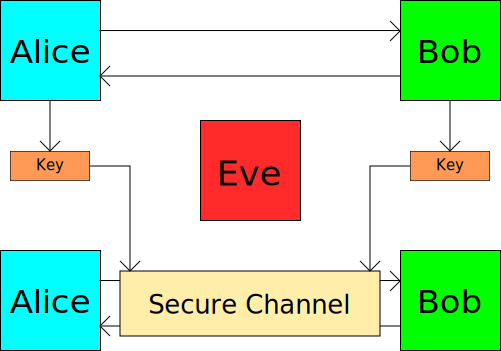
\includegraphics[width=0.6\textwidth]{out/key_exchange_problem.eps}
  \caption{Key Exchange Problem}
  \label{fig:key_exchange_problem}
\end{figure}
\FloatBarrier

\subsubsection{Trusted Third Party}

\begin{itemize}
  \item Only $\mathcal{O}(n)$ keys required
  \item No third party can be truly/fully trusted
\end{itemize}

\subsubsection{Merkle Puzzles}

\begin{itemize}
  \item Only secure against eavesdropping
  \item Only uses symmetric primitives
  \item Not used in real world applications
\end{itemize}

\begin{figure}[h!]
  \centering
  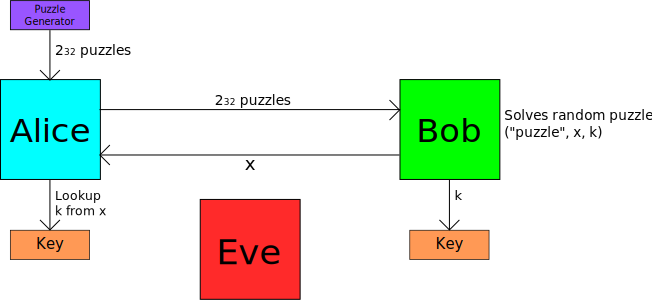
\includegraphics[width=0.8\textwidth]{out/merkle_puzzles_key_exchange.eps}
  \caption{Merkle Puzzles Key Exchange}
  \label{fig:merkle_puzzles_key_exchange}
\end{figure}
\FloatBarrier

\Para{Idea}

\begin{enumerate}
  \item[1] Alice generates a large number of puzzles (e.g. $2^{32}$) each with a
           candidate session key in the payload
  \item[2] Alice sends all the puzzles to Bob
  \item[3] Bob chooses a puzzle at random and solves it by brute force
  \item[4] Bob sends the puzzle ID back to Alice, Alice then knows which puzzle
           hence which session key Bob is using
  \item[5] Alice sends a random number $N$ to Bob, encrypted with the
           chosen session key
  \item[6] Bob replies with $N-1$ encrypted using the chosen session key
  \item[7] If the message from bob is actually $N-1$ then the key exchange was
           successful
\end{enumerate}

Choose AES key with leading zeros such that:
\[K = \{0\}^{128-l} \{0,1\}^{l}\]

Requires $2^{l}$ brute force decryption attempts to solve.

\Para{Puzzle generator}

\begin{enumerate}
  \item[1] Choose random $P \in \{0,1\}^{32}$
  \item[2] Choose random $x, k \in \{0,1\}^{128}$
  \item[3] Puzzle $P = E((\{0\}^{96}||P), "puzzle" x, k)$
\end{enumerate}

\Para{Puzzle structure}

\begin{description}
  \item[$\{0\}^{96} || P$] \hfill \\
    Random encryption key
  \item[$"puzzle" x$] \hfill \\
    Random ID
  \item[$k$] \hfill \\
    Random session key
\end{description}

\Para{Computational gap}

\begin{itemize}
  \item Workload for Alice and Bob: $\mathcal{O}(n)$, e.g. $2^{32}$
  \item Workload for Eve: $\mathcal{O}(n^{2})$, e.g. $2^{64}$
  \item Quadratic gap is best achievable for symmetric block ciphers
\end{itemize}

\subsubsection{Diffie-Hellman}

\begin{itemize}
  \item Only secure against eavesdropping
  \item Uses asymmetric primitives
\end{itemize}

\begin{figure}[h!]
  \centering
  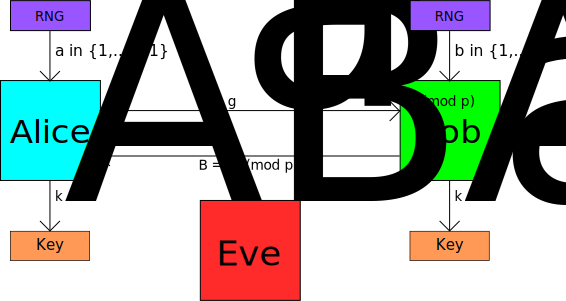
\includegraphics[width=0.6\textwidth]{out/diffie_hellman_key_exchange.eps}
  \caption{Diffe-Hellman Key Exchange}
  \label{fig:diffe_hellman_key_exchange}
\end{figure}
\FloatBarrier

\Para{Idea}

\begin{enumerate}
  \item[1] A large prime number $p$ and integer $g$ (generator of
           $(\mathbb{Z}_{p})^{*}$) are known by everyone
  \item[2] Alice chooses a random $a \in \mathbb{Z}_{p} / \{0\}$
  \item[2] Bob chooses a random $b \in \mathbb{Z}_{p} / \{0\}$
  \item[3] Alice transmits $A = g^{a} (\Mod p)$ to Bob
  \item[4] Bob transmits $B = g^{b} (\Mod p)$ to Alice
  \item[5] Alice computes session key $k_{AB} = B^{a}$
  \item[6] Bob computes session key $k_{AB} = A^{b}$
\end{enumerate}

\Para{Proof of correctness}

Proof of correctness of session keys:
\begin{align*}
  k_{AB(alice)} &= k_{AB(bob)} \\
  B^{a} &= A^{b} \\
  g^{b^{a}} &= g^{a^{b}} \\
  g^{ba} &= g^{ab} \\
  g^{ab} &= g^{ab}
\end{align*}

\Para{Difficulty}

\begin{table}[h]
  \centering
  \begin{tabular}{@{}ll@{}}
    \toprule
    Symmetric Cipher Key Size & DH/RSA Modulus Size \\
    \midrule
    80 bits                   & 1028 bits           \\
    128 bits                  & 3072 bits           \\
    \bottomrule
  \end{tabular}
  \caption{Diffie-Hellman Difficulty}
  \label{tab:diffie_hellman_difficulty}
\end{table}
\FloatBarrier

Best known algorithm to break DH/RSA is General Number Field Sieve, the expected
running time of which is $\mathcal{O}(exp(log(N)^{\frac{1}{3}}))$.

\subsubsection{Establishing a secure channel}

\begin{itemize}
  \item Messages are sent encrypted with a symmetric cipher with a MAC
  \item Avoid using same key for all ciphers and MAC generation by using key
        derivation
\end{itemize}

\begin{figure}[h!]
  \centering
  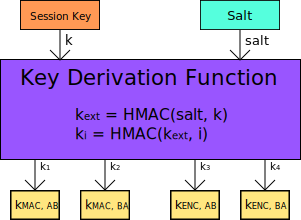
\includegraphics[width=0.6\textwidth]{out/key_derivation_function.eps}
  \caption{Key Derivation Function}
  \label{fig:key_derivation_function}
\end{figure}
\FloatBarrier

Key derivation generates different keys for cipher and MAC in both directions (4
unique keys in total) using the session key and a known salt.

\subsection{Public Key Encryption}

\subsubsection{RSA}

TODO

\subsubsection{ElGamal}

TODO

\subsection{Digital Signatures}

\subsubsection{RSA}

TODO

\subsection{Zero Knowledge Proofs}

TODO

\end{document}
